\documentclass[11pt,a4paper]{article}
\usepackage{fontspec}
\usepackage[french]{babel}
\usepackage[margin=2.2cm]{geometry}
\usepackage{graphicx}
\usepackage{booktabs}
\usepackage{array}
\usepackage{xcolor}
\usepackage{amsmath}
\usepackage{enumitem}
\usepackage{float}
\usepackage[hidelinks]{hyperref}
\usepackage{titlesec}
\usepackage{fancyhdr}

\definecolor{navy}{HTML}{1F3864}
\definecolor{ib}{HTML}{2E75B6}
\titleformat{\section}{\Large\bfseries\color{navy}}{\thesection}{0.8em}{}
\titleformat{\subsection}{\large\bfseries\color{ib}}{\thesubsection}{0.6em}{}
\setlist{itemsep=2pt,topsep=4pt}
\graphicspath{{../analyses/001_pernod_ricard/exhibits/}}

\pagestyle{fancy}\fancyhf{}
\lhead{\small\color{navy}Projet Axone — Synthèse}
\rhead{\small\thepage}
\renewcommand{\headrulewidth}{0.4pt}

\emergencystretch=3em
\newcommand{\eur}{\,€}

\title{\color{navy}\textbf{Projet Axone}\\[4pt]\large Recherche actions indépendante — synthèse du projet}
\author{Dossier \texttt{axone/}}
\date{Octobre 2026}

\begin{document}
\maketitle
\thispagestyle{fancy}

\begin{center}
\fbox{\parbox{0.9\linewidth}{\small
\textbf{En une phrase.} Axone est une mini-plateforme de \emph{equity research} indépendante :
un site web vitrine (HTML/CSS/JS) qui publie, une fois par mois, une analyse de valorisation
d'une société cotée réalisée « comme en banque d'affaires » (DCF, comparables boursiers,
transactions précédentes, football field), avec le modèle Excel et le pitchbook PowerPoint en
téléchargement. Première valeur couverte : \textbf{Pernod Ricard (RI FP)} — recommandation
\textbf{BUY}, objectif \textbf{108\eur} contre un cours de 64,14\eur (+68\,\%).}}
\end{center}

\tableofcontents
\newpage

%=====================================================================
\section{À quoi sert le projet ?}
Axone a un double objectif :
\begin{itemize}
  \item \textbf{Vitrine / portfolio} : démontrer des compétences d'analyste (banque d'affaires,
        recherche actions, M\&A) à travers des livrables professionnels publiés ouvertement.
  \item \textbf{Publication de recherche} : une analyse approfondie par mois, entièrement bâtie à
        partir de documents publics, avec un modèle « open book » (toutes les hypothèses,
        bridges et sensibilités sont visibles).
\end{itemize}
Le site précise qu'il s'agit d'un contenu \emph{à but pédagogique}, ni conseil en
investissement ni sollicitation.

\paragraph{Pipeline annoncé.} Après Pernod Ricard : LVMH (somme des parties), ASML
(semi-conducteurs, monopole EUV vs cyclicité et restrictions d'export), puis une banque
(BNP Paribas / Société Générale) valorisée en P/B vs ROE, DDM et P/E plutôt qu'en DCF.

%=====================================================================
\section{Que contient le dossier ?}
\begin{table}[H]\centering\small
\begin{tabular}{>{\raggedright\arraybackslash}p{5.6cm}p{9.6cm}}
\toprule
\textbf{Élément} & \textbf{Rôle} \\
\midrule
\texttt{index.html}, \texttt{css/}, \texttt{js/main.js} & Site statique « one-page » : présentation, couverture, analyse phare, méthodologie, pipeline, newsletter, contact. \\
\texttt{assets/docs/} & Pitchbook \texttt{.pptx} et modèle \texttt{.xlsx} proposés au téléchargement. \\
\texttt{assets/img/}, \texttt{assets/fonts/} & 12 graphiques (exhibits), favicon, police Inter. \\
\texttt{001\_pernod\_ricard/docs/} & Sources : URD 2023-24 et 2024-25, états financiers consolidés, rapports de gestion, communiqués H1 et 9M FY26, tableaux de dette nette. \\
\texttt{001\_pernod\_ricard/*.xlsx} & Modèle de valorisation (v1, v1 macro \texttt{.xlsm}, v2 finale). \\
\texttt{001\_pernod\_ricard/exhibits/} & Les 12 graphiques PNG du pitchbook. \\
\texttt{analyses/000\_script/} & Scripts Python d'automatisation (voir §\ref{sec:tech}). \\
\bottomrule
\end{tabular}
\end{table}

%=====================================================================
\section{Stack technique}\label{sec:tech}
\subsection{Site web}
\begin{itemize}
  \item HTML/CSS/JavaScript \textbf{vanilla}, sans framework ni dépendance externe.
  \item Fonctionnalités JS : bilingue EN/FR (dictionnaire i18n), thème clair/sombre mémorisé en
        \texttt{localStorage}, menu burger, \emph{scroll-spy}, animations d'apparition, compteurs
        animés (prix cible, upside, WACC), barre de pondération des méthodes, galerie + lightbox
        des 12 exhibits.
  \item Formulaire newsletter envoyé via le service \texttt{formsubmit.co} (AJAX).
\end{itemize}

\subsection{Chaîne d'analyse (Python)}
\begin{enumerate}
  \item \texttt{format\_banking\_conventions.py} — applique au modèle Excel les conventions de
        banque : \textcolor{blue}{bleu = input}, noir = formule, \textcolor{green!50!black}{vert = lien
        inter-onglets}, formats de nombres (négatifs entre parenthèses, multiples en « x »,
        pourcentages). Purement cosmétique, idempotent, avec sauvegarde horodatée
        (\texttt{openpyxl}).
  \item \texttt{export\_charts.py} — lit les valeurs du modèle et régénère les 12 graphiques en
        PNG (\texttt{matplotlib}, charte « bulge bracket »).
  \item \texttt{build\_pitchbook.py} — assemble le pitchbook de 12 slides au format banque
        (\texttt{python-pptx}) : bandeau navy, sources en pied de page, « key takeaways ».
\end{enumerate}
\noindent Chaîne : \textbf{PDF publics $\rightarrow$ modèle Excel $\rightarrow$ graphiques
$\rightarrow$ pitchbook $\rightarrow$ site}.

\subsection{Le modèle Excel (v2) — 12 onglets}
\texttt{Cover} (synthèse/recommandation), \texttt{Data} (données de marché sourcées et datées),
\texttt{Assumptions}, \texttt{Income\_Statement} (FY23–FY25), \texttt{DCF}, \texttt{WACC},
\texttt{Bridge} (EV $\rightarrow$ equity), \texttt{Sensitivity}, \texttt{Trading\_Comps},
\texttt{Precedent\_Transactions}, \texttt{Football\_Field}, \texttt{Chart\_Data}.

%=====================================================================
\section{Notions financières mobilisées}

\subsection{Lecture des états financiers}
\begin{itemize}
  \item \textbf{Compte de résultat} Pernod Ricard : chiffre d'affaires net, marge brute (après
        logistique), \textbf{A\&P} (dépenses publicitaires et promotionnelles), coûts de
        structure, \textbf{ROC / PRO} (\emph{Profit from Recurring Operations}, utilisé comme
        EBIT), résultat net part du groupe, BPA dilué.
  \item \textbf{EBITDA} $=$ PRO $+$ D\&A. Marges : brute ~60\,\%, PRO ~27\,\%, EBITDA ~31\,\%.
  \item \textbf{Croissance organique} (hors effets de change et de périmètre) vs publiée ;
        \textbf{rebasing} de périmètre ($-4{,}8\,\%$ pour les cessions Vins et Imperial Blue).
  \item \textbf{Dette nette en IFRS 16} (inclut les dettes locatives), intérêts minoritaires,
        sociétés mises en équivalence.
\end{itemize}

\subsection{DCF (Discounted Cash Flow)}
Projection sur 5 ans (FY26E–FY30E) par région (Amériques, Asie/RdM, Europe), puis :
\[
\text{FCF}_{\text{unlevered}} = \underbrace{\text{EBIT}\times(1-t)}_{\text{NOPAT}} + \text{D\&A} - \text{Capex} - \Delta\text{BFR},
\qquad t = 25\,\% \text{ (normatif)}
\]
\[
\text{EV} = \sum_{n=1}^{5}\frac{\text{FCF}_n}{(1+\text{WACC})^n} + \frac{\text{TV}}{(1+\text{WACC})^5}
\]
Deux méthodes de \textbf{valeur terminale} :
\begin{itemize}
  \item \textbf{Gordon-Shapiro} (croissance à l'infini) :
        $\text{TV} = \dfrac{\text{FCF}_{5}\,(1+g)}{\text{WACC}-g}$ avec $g = 1{,}5\,\%$ ;
  \item \textbf{Multiple de sortie} : $\text{TV} = \text{EBITDA}_{\text{FY30}} \times 11{,}0\text{x}$.
\end{itemize}

\subsection{WACC et CAPM}
\[
K_e = r_f + \beta \times \text{ERP} = 3{,}74\,\% + 1{,}25\times 5{,}5\,\% = 10{,}6\,\%
\]
\[
\text{WACC} = \frac{E}{V}K_e + \frac{D}{V}K_d(1-t) = 59{,}1\,\%\times10{,}6\,\% + 40{,}9\,\%\times 3{,}2\,\%\times 0{,}75 \approx 7{,}25\,\%
\]
$r_f$ = OAT 10 ans, ERP France (Damodaran), $K_d$ = coût moyen de la dette (notation BBB+/Baa1),
pondérations en valeur de marché.

\subsection{Pont EV $\rightarrow$ valeur des fonds propres (equity bridge)}
\[
\text{Equity} = \text{EV} - \text{Dette nette} - \text{Minoritaires} + \text{Participations},
\qquad \text{Prix/action} = \frac{\text{Equity}}{\text{Nb d'actions diluées}}
\]

\subsection{Méthodes par multiples}
\begin{itemize}
  \item \textbf{Comparables boursiers} (\emph{trading comps}) : EV/EBITDA, EV/Ventes, P/E de
        Diageo, Rémy Cointreau, Campari, Brown-Forman, Becle (Cuervo), Constellation Brands ;
        médiane, moyenne, quartiles Q1/Q3.
  \item \textbf{Transactions précédentes} : multiples payés lors d'acquisitions de contrôle
        (Beam par Suntory, Absolut, Allied Domecq, Grand Marnier, Courvoisier\dots) — ils
        intègrent une \textbf{prime de contrôle}.
\end{itemize}

\subsection{Synthèse et analyse de risque}
\begin{itemize}
  \item \textbf{Football field} : fourchettes de valeur par méthode comparées au cours, au range
        52 semaines et au consensus.
  \item \textbf{Prix cible pondéré} : 50\,\% DCF, 35\,\% comps, 15\,\% précédents.
  \item \textbf{Analyse de sensibilité} à deux entrées : WACC $\times$ $g$, et WACC $\times$
        multiple de sortie.
  \item \textbf{Levier} : dette nette / EBITDA, conversion de cash, politique de dividende
        (DPA 4,70\eur), notation de crédit.
\end{itemize}

%=====================================================================
\section{Résultats : l'analyse Pernod Ricard}

\subsection{Données clés (juin 2026)}
\begin{table}[H]\centering\small
\begin{tabular}{lr@{\hspace{1.5cm}}lr}
\toprule
Cours & 64,14\eur & Capitalisation & 16,1\,Md\eur \\
Actions & 251,6\,M & Dette nette (IFRS 16) & 11,2\,Md\eur \\
Valeur d'entreprise & 27,3\,Md\eur & EV/EBITDA FY25 & 8,1x \\
CA FY25 & 10,96\,Md\eur & PRO FY25 & 2,95\,Md\eur (26,9\,\%) \\
\bottomrule
\end{tabular}
\end{table}

\subsection{Valorisation par méthode}
\begin{table}[H]\centering\small
\begin{tabular}{lrr}
\toprule
\textbf{Méthode} & \textbf{Prix implicite} & \textbf{Poids} \\
\midrule
DCF — Gordon ($g=1{,}5\,\%$) & 88,46\eur & \\
DCF — Multiple de sortie (11,0x) & 99,41\eur & \\
\quad DCF (moyenne) & 93,94\eur & 50\,\% \\
Comparables (médiane 12,4x EV/EBITDA FY26E) & 105,06\eur & 35\,\% \\
Précédents (médiane 16,9x) & 161,12\eur & 15\,\% \\
\midrule
\textbf{Prix cible pondéré} & \textbf{107,91\eur} & \textbf{+68\,\%} \\
\bottomrule
\end{tabular}
\end{table}

\begin{figure}[H]\centering
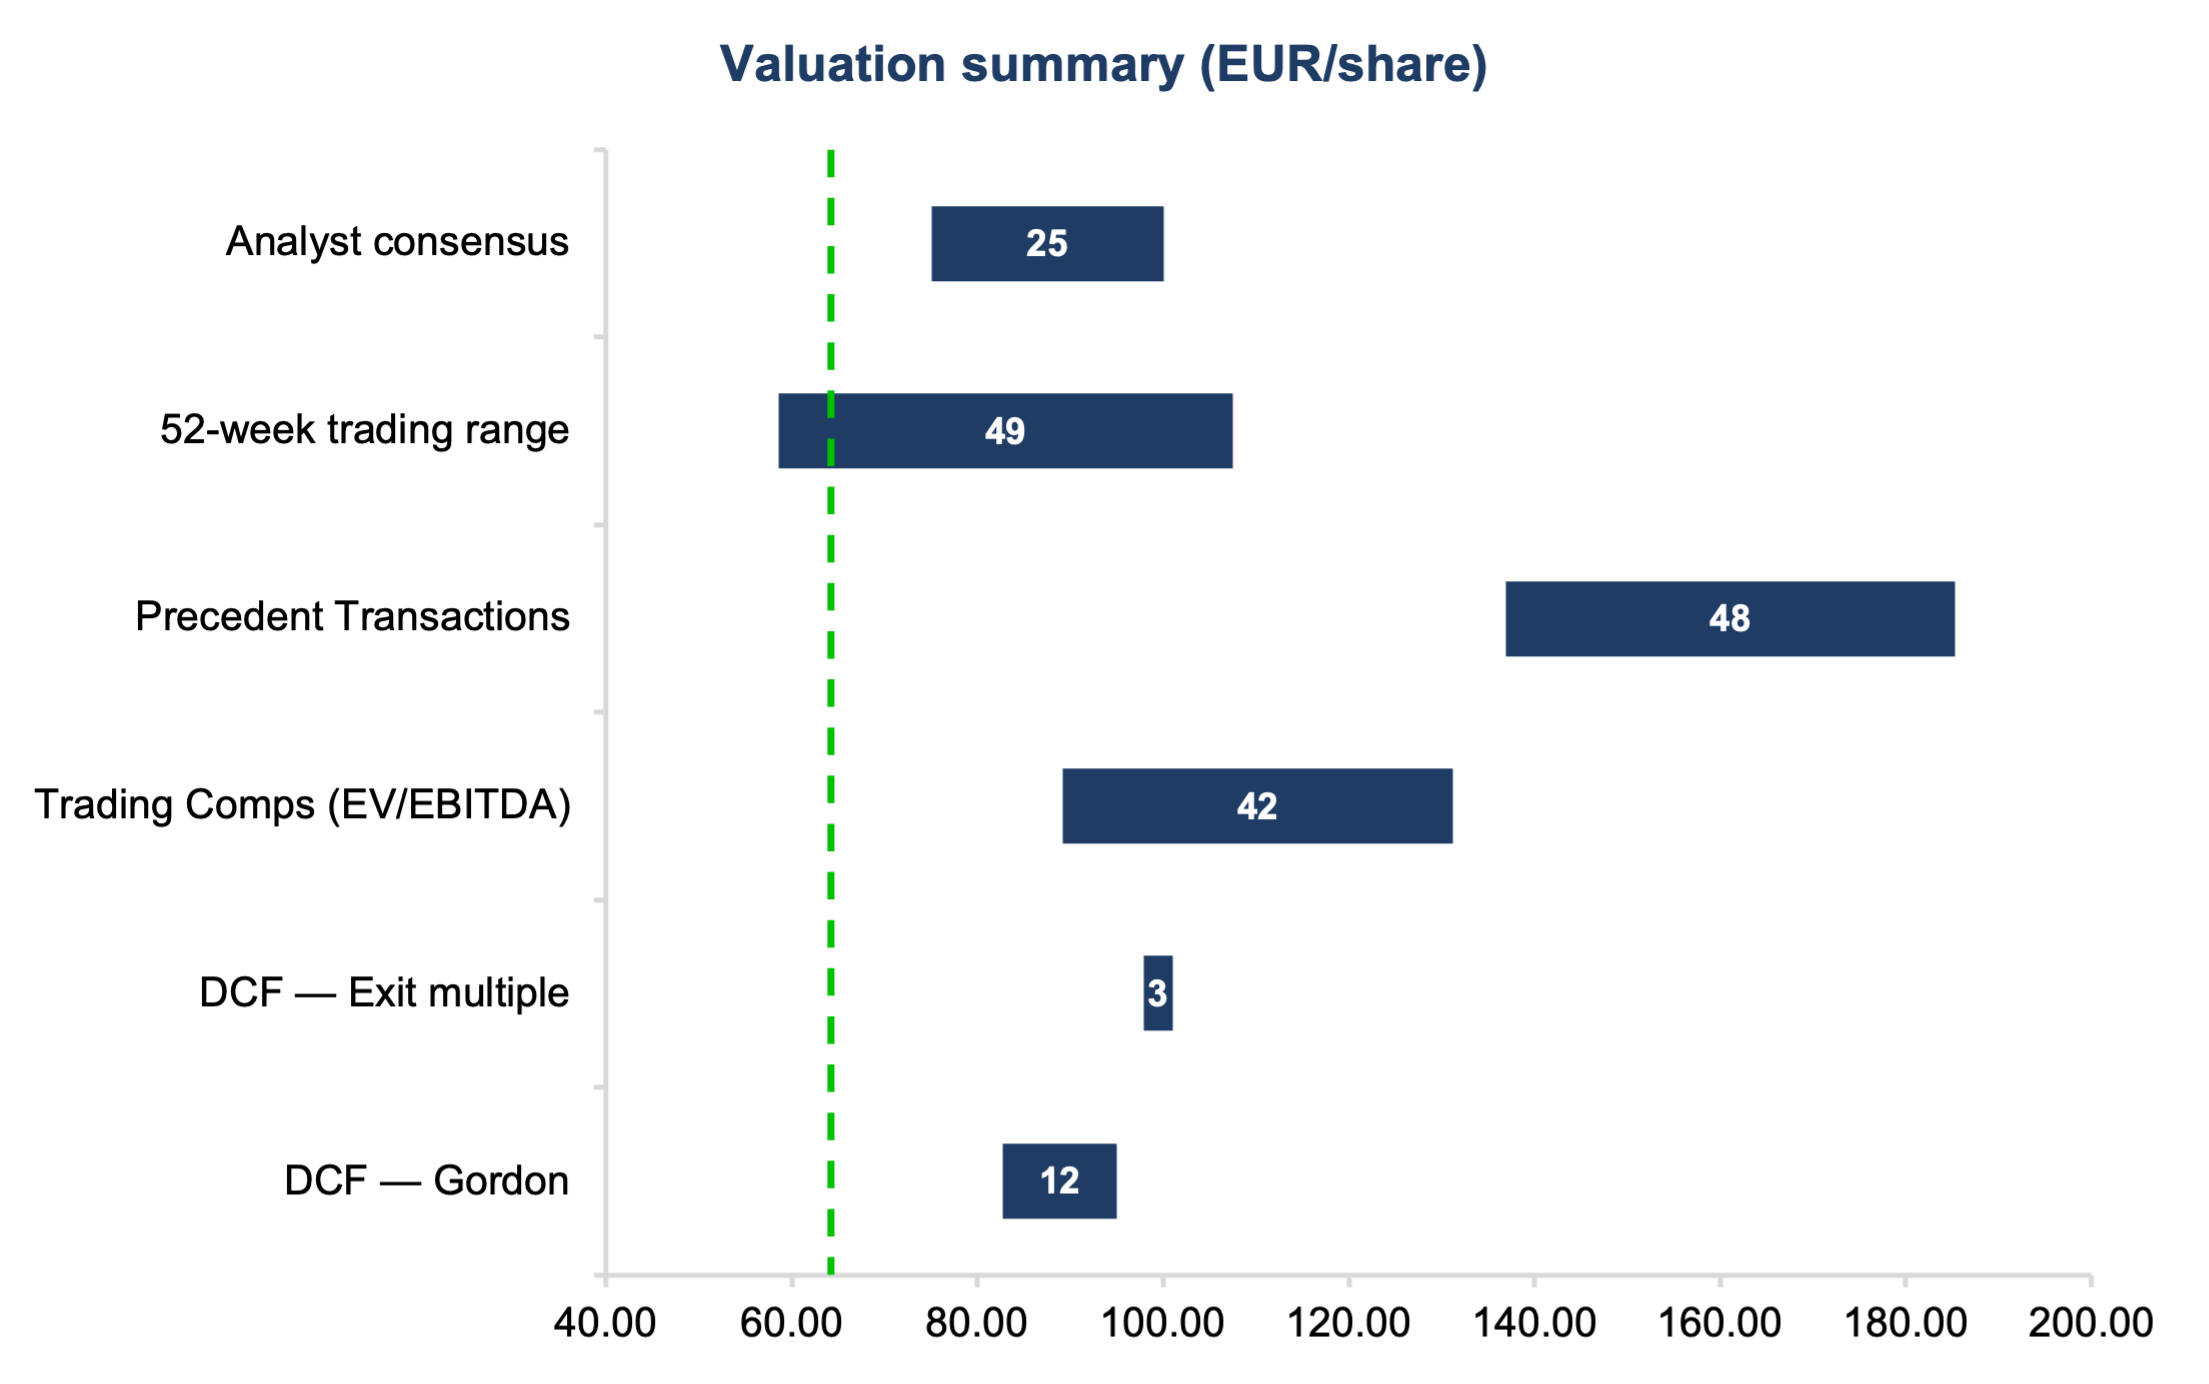
\includegraphics[width=0.78\linewidth]{chart_01.png}
\caption{Football field (exhibit 1 du pitchbook). Ligne verte : cours actuel.}
\end{figure}

\subsection{Thèse d'investissement}
\begin{enumerate}
  \item \textbf{Décote de valorisation} : 8,1x EV/EBITDA contre une médiane de pairs de 12,4x,
        malgré une position de n°2 mondial et des marques premium (Jameson, Absolut, Martell,
        Chivas).
  \item \textbf{FY26 année de transition} : ventes organiques T3 à +0,1\,\% après un S1 faible ;
        guidance +3 à +6\,\% organique par an sur FY27–29.
  \item \textbf{Désendettement} : dette nette/EBITDA de ~3,45x (FY26E) à ~2,0x (FY30E).
  \item \textbf{Valeur spéculative M\&A} : les transactions du secteur (~16,9x) impliquent une
        valeur de contrôle bien supérieure à l'objectif.
\end{enumerate}

\subsection{Principales hypothèses}
Croissance FY26E : Amériques $-9\,\%$, Asie $-1\,\%$, Europe $-1\,\%$, puis reprise
(+4/5\,\% sur Amériques et Asie). Marge brute 59\,\% $\rightarrow$ 60\,\%, A\&P stable à 16\,\%,
coûts de structure 16\,\% $\rightarrow$ 15\,\% (plan d'efficacité de 1\,Md\eur), capex 5–5,5\,\% du CA.
Marge PRO : 27,0\,\% (FY26E) $\rightarrow$ 29,0\,\% (FY30E).

\subsection{Risques identifiés}
Chine (cognac/Martell, enquêtes antidumping UE–Chine), normalisation des stocks aux
États-Unis, change (USD, INR, TRY), Travel Retail, exécution du plan d'efficacité, tarifs
douaniers.

\begin{figure}[H]\centering
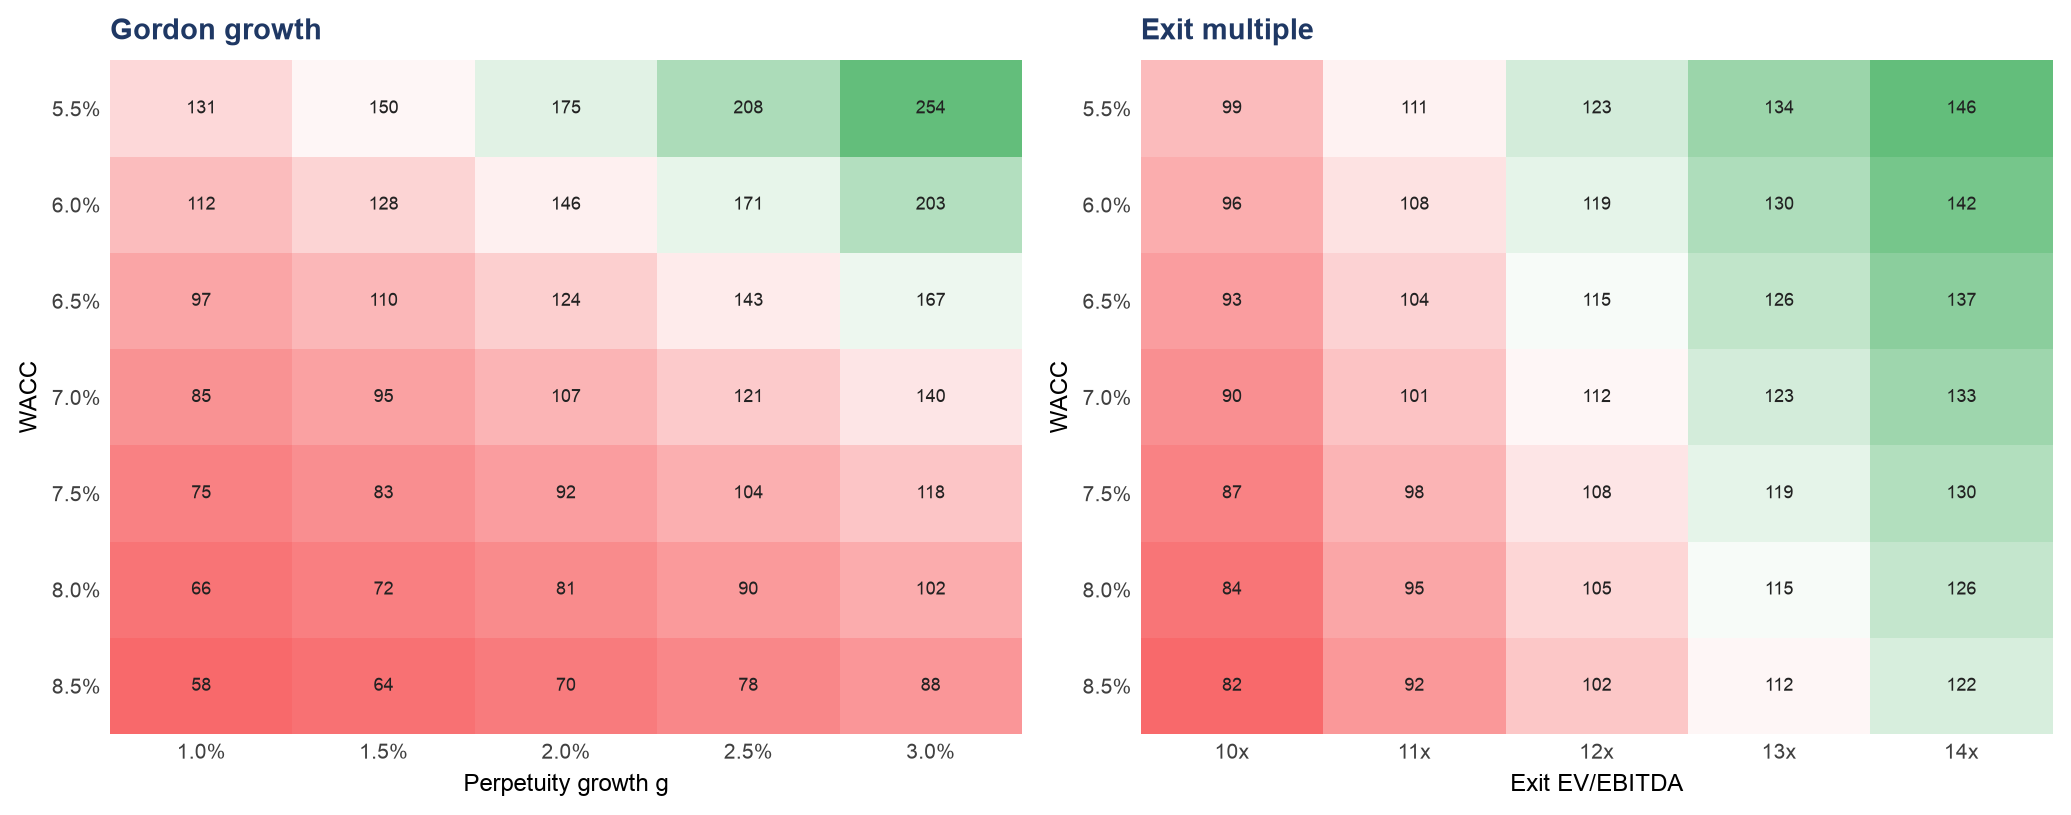
\includegraphics[width=0.75\linewidth]{chart_12.png}
\caption{Sensibilité du DCF au WACC, à $g$ et au multiple de sortie (exhibit 12).}
\end{figure}

%=====================================================================
\section{Regard critique : points à vérifier}
L'analyse est solide dans sa structure. Quelques points mériteraient d'être revus avant
diffusion à un recruteur ou à un lecteur exigeant :
\begin{itemize}
  \item \textbf{Bêta} : le bêta brut de marché saisi est de 0,38, mais le WACC utilise 1,25 sans
        justification visible (pas de dé-/ré-endettement des bêtas des pairs). C'est le
        paramètre le plus sensible du modèle.
  \item \textbf{Poids de la valeur terminale} : la VT actualisée représente ~78\,\% de l'EV
        (Gordon). Le multiple implicite de la VT Gordon est ~10,0x l'EBITDA FY30, inférieur au
        multiple de sortie retenu (11,0x) — d'où l'écart entre les deux DCF.
  \item \textbf{Incohérence de décote} : le site parle d'une décote de « ~24\,\% » vs la médiane
        des pairs, alors que $1 - 8{,}1/12{,}4 \approx 35\,\%$ (24--25\,\% correspond à la
        décote vs Diageo seul). Le pitchbook, lui, mentionne ~35\,\%.
  \item \textbf{Précédents présentés comme un « plancher »} : un multiple de transaction inclut une
        prime de contrôle ; le présenter comme plancher de valorisation est agressif. Deux des
        sept transactions (Casamigos, Wilderness Trail) n'ont pas de données.
  \item \textbf{Comparables} : EBITDA FY26E de Pernod rapporté aux multiples des pairs dont la base
        (historique/prévisionnelle) n'est pas précisée ; légers écarts dans la ligne « self »
        (11\,200 vs 11\,168\,M\eur de dette nette, 251,8 vs 251,6\,M actions).
  \item \textbf{Sensibilité} : le scénario « stressé » (WACC 8\,\%, $g$ 1\,\%) donne 65,5\eur, à
        peine au-dessus du cours ; à 8,5\,\% de WACC la valeur passe sous le cours.
  \item \textbf{Coût de la dette} : 3,2\,\% (moyen historique) alors que le coût marginal indiqué
        est 3,25–3,75\,\%.
\end{itemize}

%=====================================================================
\section{Conclusion}
Axone combine un \textbf{site web statique soigné}, une \textbf{chaîne d'automatisation Python}
(Excel $\rightarrow$ graphiques $\rightarrow$ PowerPoint) et un \textbf{modèle de valorisation
complet} selon les standards de la banque d'affaires. Le projet couvre l'essentiel de la
boîte à outils de l'analyste : analyse financière, DCF, WACC/CAPM, multiples boursiers et de
transaction, bridge EV/equity, sensibilités et levier. La première étude conclut à un
\textbf{BUY sur Pernod Ricard, objectif 108\eur (+68\,\%)}.

\end{document}
